\section{QUARKONIA}
\label{quarkonia}
Quarkonium production is believed to give important information about the
hot and dense matter formed in heavy-ion collisions.
The in-medium suppression  of quarkonium states caused by Debye screening of the color potential between heavy quarks
is expected to depend on the their binding energy and the temperature of the medium, leading to a sequential
disappearance of the various charmonium and
bottomonium states~as the temperature increases\cite{Matsui:1986dk,Digal:2001ue,Mocsy:2007jz}. Therefore, the measurement of the quarkonium suppression pattern is sometimes called the QGP thermometer. At the increase of the temperature, first the higher-mass (less bound) states, such as \psip\ and \PgUc\, are melted, then \Jpsi\ and \PgUb\ at approximately the same point, and finally the most tightly bound \PgUa\ is expected to disappear only at very high temperature (about twice the critical temperature). However, a significant fraction of the lower-mass states is normally produced as a decay product of the higher-mass states, including those difficult to observed directly, e.g. \chic\ and $\chi_{\rm b}$, therefore \Jpsi\ and \PgUa\ can be suppressed even if their corresponding melting temperatures are not reached.

Suppression of \Jpsi\ production was clearly observed in central heavy-ion collisions at CERN SPS~\cite{Baglin:1994ui,Alessandro:2004ap,Alessandro:2006ju,Arnaldi:2007zz}, and an effect on about the same level was later measured at RHIC~\cite{Adare:2006ns,Adare:2011yf}. The quantitative interpretation of the observed suppression is complicated by cold nuclear-matter effects, such as the modification of nuclear structure functions and final state absorption. At higher collision energies, when the production of charm becomes more abundant, the charmonium states can be regenerated~\cite{BraunMunzinger:2000px,Thews:2000rj,Andronic:2007bi,Zhao:2007hh,Capella:2007jv}. At the LHC in a central Pb--Pb collision ${\cal O}(100)$ c$\overline{\rm c}$ pairs are produced, and they may recombine during the hadronization into charmonia, thus compensating the initial suppression. The regeneration yield is strongly dependent on  the c$\overline{\rm c}$ quark density, and therefore can be inferred from the measurement in different kinematical regions and at different collision energies. At the LHC energies the feed-down of charmonium states from B-hadron decays is sizeable. This can be exploited for B-production measurements, as explained in Sec.~\ref{subsecks:heavyspectra}, and data for charmonium production are presented corrected for such feed-down, i.e prompt J/$\psi$, or without this correction, i.e. inclusive J/$\psi$.

The large advantage brought by the LHC energy is the increase of the quarkonium cross sections, and this is especially beneficial for $\Upsilon$ family allowing for high statistics measurement for the first time. The three observed $\Upsilon$ states have very similar initial conditions, therefore the expected suppression pattern reflects the hierarchy of their binding energies, with possible (small) absorption corrections. The regeneration effect in this case will be negligible, due to order of magnitude lower b-quark density compared to that of c quarks.

\subsection{Charmonium Production}

The ATLAS and CMS experiments are measuring \Jpsi\ production in the dimuon channel for relatively high $p_{\rm T}$~\cite{Aad:2010aa,Chatrchyan:2012np}, above 3--6.5~GeV, depending on the rapidity range. ALICE is capable to detect charmonia down to zero \pT\ both in the dimuon channel in forward region ($2.5 < y < 4$)~\cite{Abelev:2012rv}, and in the dielectron channel in the mid-rapidity region ($|y| < 0.9$)~\cite{Abelev:2013ila}. The results are usually presented in terms of the nuclear modification factor, $R_{\rm AA}$, defined in Eq.~\ref{eqks:RAA}.

The rapidity dependence of the inclusive \Jpsi\ $R_{\rm AA}$, integrated over centrality and $p_{\rm T} > 0$ (or $> 3$~GeV)~\cite{Abelev:2012rv,Abelev:2013ila}, does not show a strong variation up to $y = 3$ and the $R_{\rm AA}$ is around 0.7 for $p_{\rm T} > 0$. At higher rapidities, up to $y = 4$, there is a tendency for more suppression, the $R_{\rm AA}$ value decreases down to 0.4. At higher \pT\ ($> 6.5$~GeV), the \Jpsi\ suppression is stronger, and was measured separately for prompt and non-prompt \Jpsi~\cite{Chatrchyan:2012np,CMS:2012wba}, with the centrality and \pT\ integrated \Raa\ found to be about 20\,\% lower for prompt than for non-prompt \Jpsi.

\begin{figure}[!ht]
\begin{center}
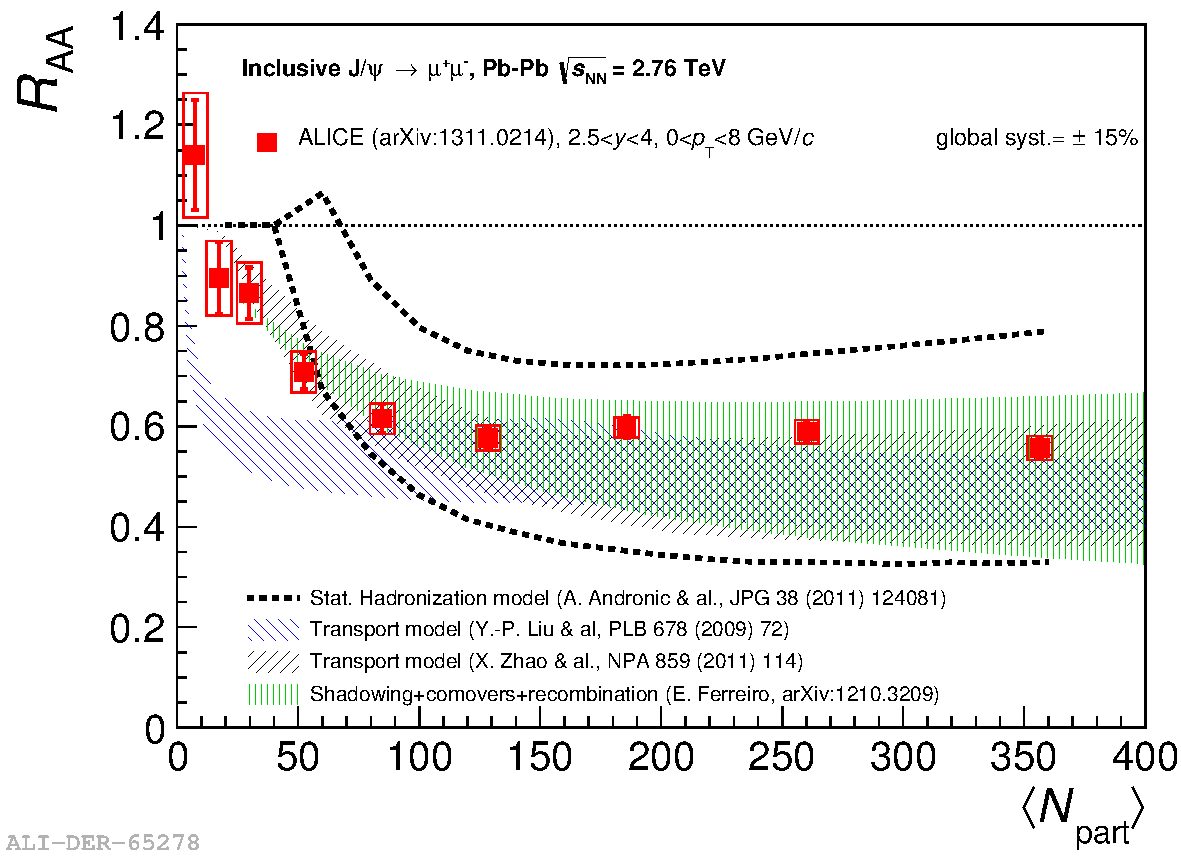
\includegraphics[width=0.49\linewidth]{quarkoniafigs/JpsiRAAcentrality.pdf}
\label{fig:KS:RaavsCent} 
\caption{Inclusive \jpsi\ \Raa\ measured in \PbPb\
collisions at $\rootsNN = 2.76$\TeV\ as a function of $N_{part}$ for two \pT\ ranges.
Total systematic uncertainties are displayed as open boxes.The experimental measurements are compared with
model calculations~\cite{Andronic:2011yq,Liu:2009nb,Zhao:2011cv,Ferreiro:2012rq}, which all include \Jpsi\ regeneration effects. Figure adapted from~\cite{Abelev:2012rv}.}
\end{center}
\end{figure}

In the forward rapidity region ($2.5 < y < 4$) detailed measurements of the \Jpsi\ \Raa\ were performed by ALICE. The centrality dependence, expressed as a function of $N_{\rm part}$, is presented in Fig.~\ref{fig:KS:RaavsCent} for $\pt > 0$. For $N_{\rm part} > 100$ (corresponding to about 40\,\% most central collisions) the inclusive \Jpsi\ suppression is approximately constant, with \Raa\ about 0.5--0.6. Moving to more peripheral collisions, the nuclear modification factor increases progressively eventually becoming consistent with unity. This centrality behavior is qualitatively different compared to that measured in forward region by PHENIX~\cite{Adare:2011yf}. At RHIC the \Jpsi\ nuclear modification factor steadily decreases with increasing $N_{\rm part}$, falling to 0.2 for most central collisions, which means almost three times stronger \Jpsi\ suppression compared to central LHC collisions.

CMS measured the centrality evolution of the \Jpsi\ suppression at $\pt > 6.5$~GeV and at mid-rapidity $|y| < 2.4$~\cite{Chatrchyan:2012np,CMS:2012wba}; the result for the prompt \Jpsi\ \Raa\ at this higher \pt\ resemble the (low-\pt) RHIC observation. Even though the non-prompt (B-decay) \Jpsi\ are less suppressed than the prompt ones, and hence the feed-down correction would decrease the inclusive \Raa\ values, this will not qualitatively affect the conclusion about the difference between RHIC and the LHC. This correction for the relevant centralities and \pt, estimated using the difference between the non-prompt and prompt \Raa\ and the measured fraction of B-decay \Jpsi\ at the LHC~\cite{Khachatryan:2010yr,Aaij:2011jh,Aad:2011sp,Chatrchyan:2012np,Abelev:2012gx}, is below 10\,\%, and only a few percents at lower \pt.

The observed suppression is stronger than that predicted for shadowing effects in the Color Singlet
Model~\cite{Ferreiro:2011rw} and the Color Evaporation Model~\cite{Vogt:2010aa}. Neither of these models predicts a strong rapidity dependence. A stronger initial-state suppression has been calculated in the Color Glass Condensate
(CGC) model~\cite{Dominguez:2011cy}, predicting  \jpsi\ \Raa\ about 0.5. However, important information is provided by the \pT\ dependence of \Jpsi\ suppression. Initial state suppression models typically lead
to a stronger suppression at lower \pT. Contrary to this, \Jpsi\ regeneration effects in statistical-hadronization~\cite{BraunMunzinger:2000px,Thews:2000rj} and in partonic-transport~\cite{{Zhao:2007hh},{Liu:2009nb}} models are expected to enhance \Jpsi\ yields at low \pT\ due to the higher phase-space density of charm quarks there. The calculations obtained with models including \Jpsi\ regeneration are compared to the (low-\pt dominated) \Jpsi\ \Raa\ measurement in Fig.~\ref{fig:KS:RaavsCent}, and they overall describe data rather well, especially for semi-peripheral to central collisions.

\begin{figure}[!ht]
\begin{center}
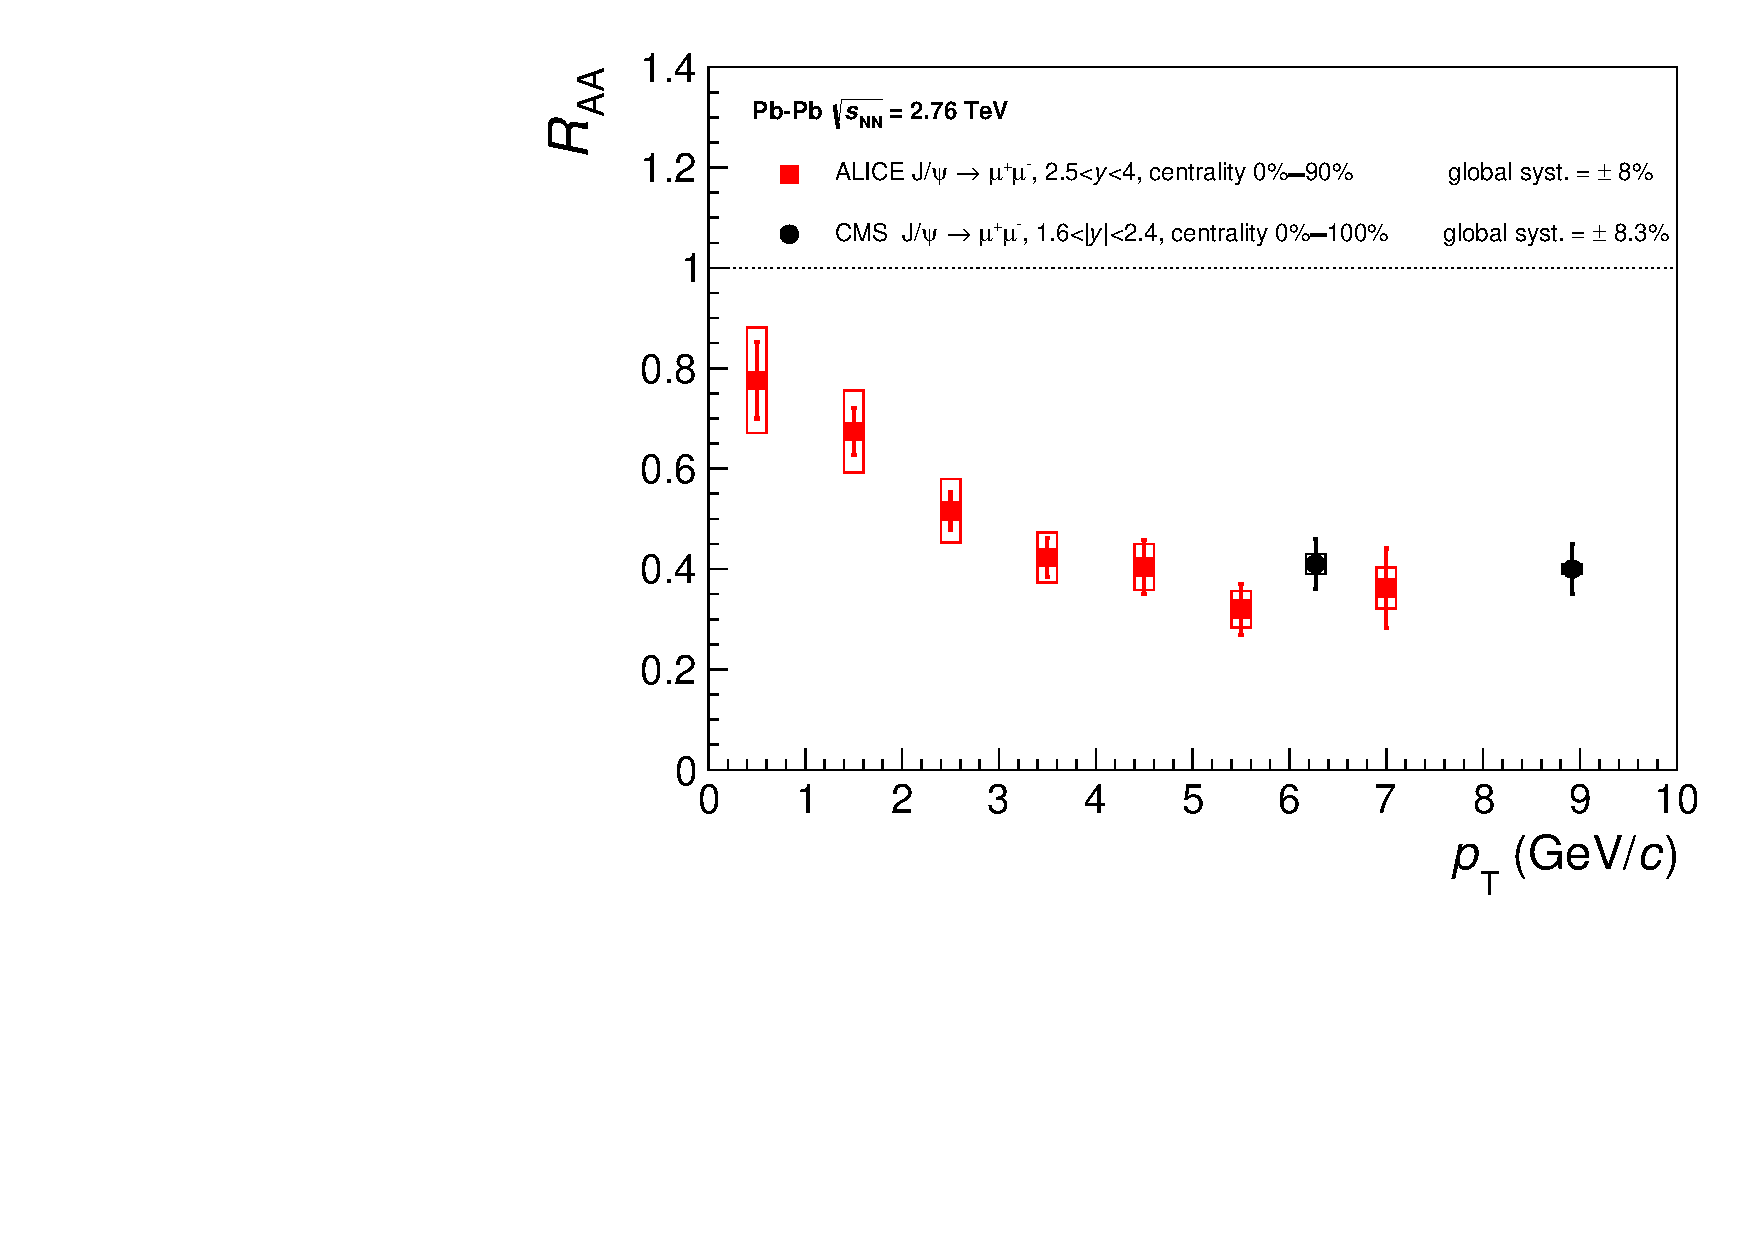
\includegraphics[width=0.49\linewidth,keepaspectratio]{quarkoniafigs/RAAPtvsModels1.pdf}
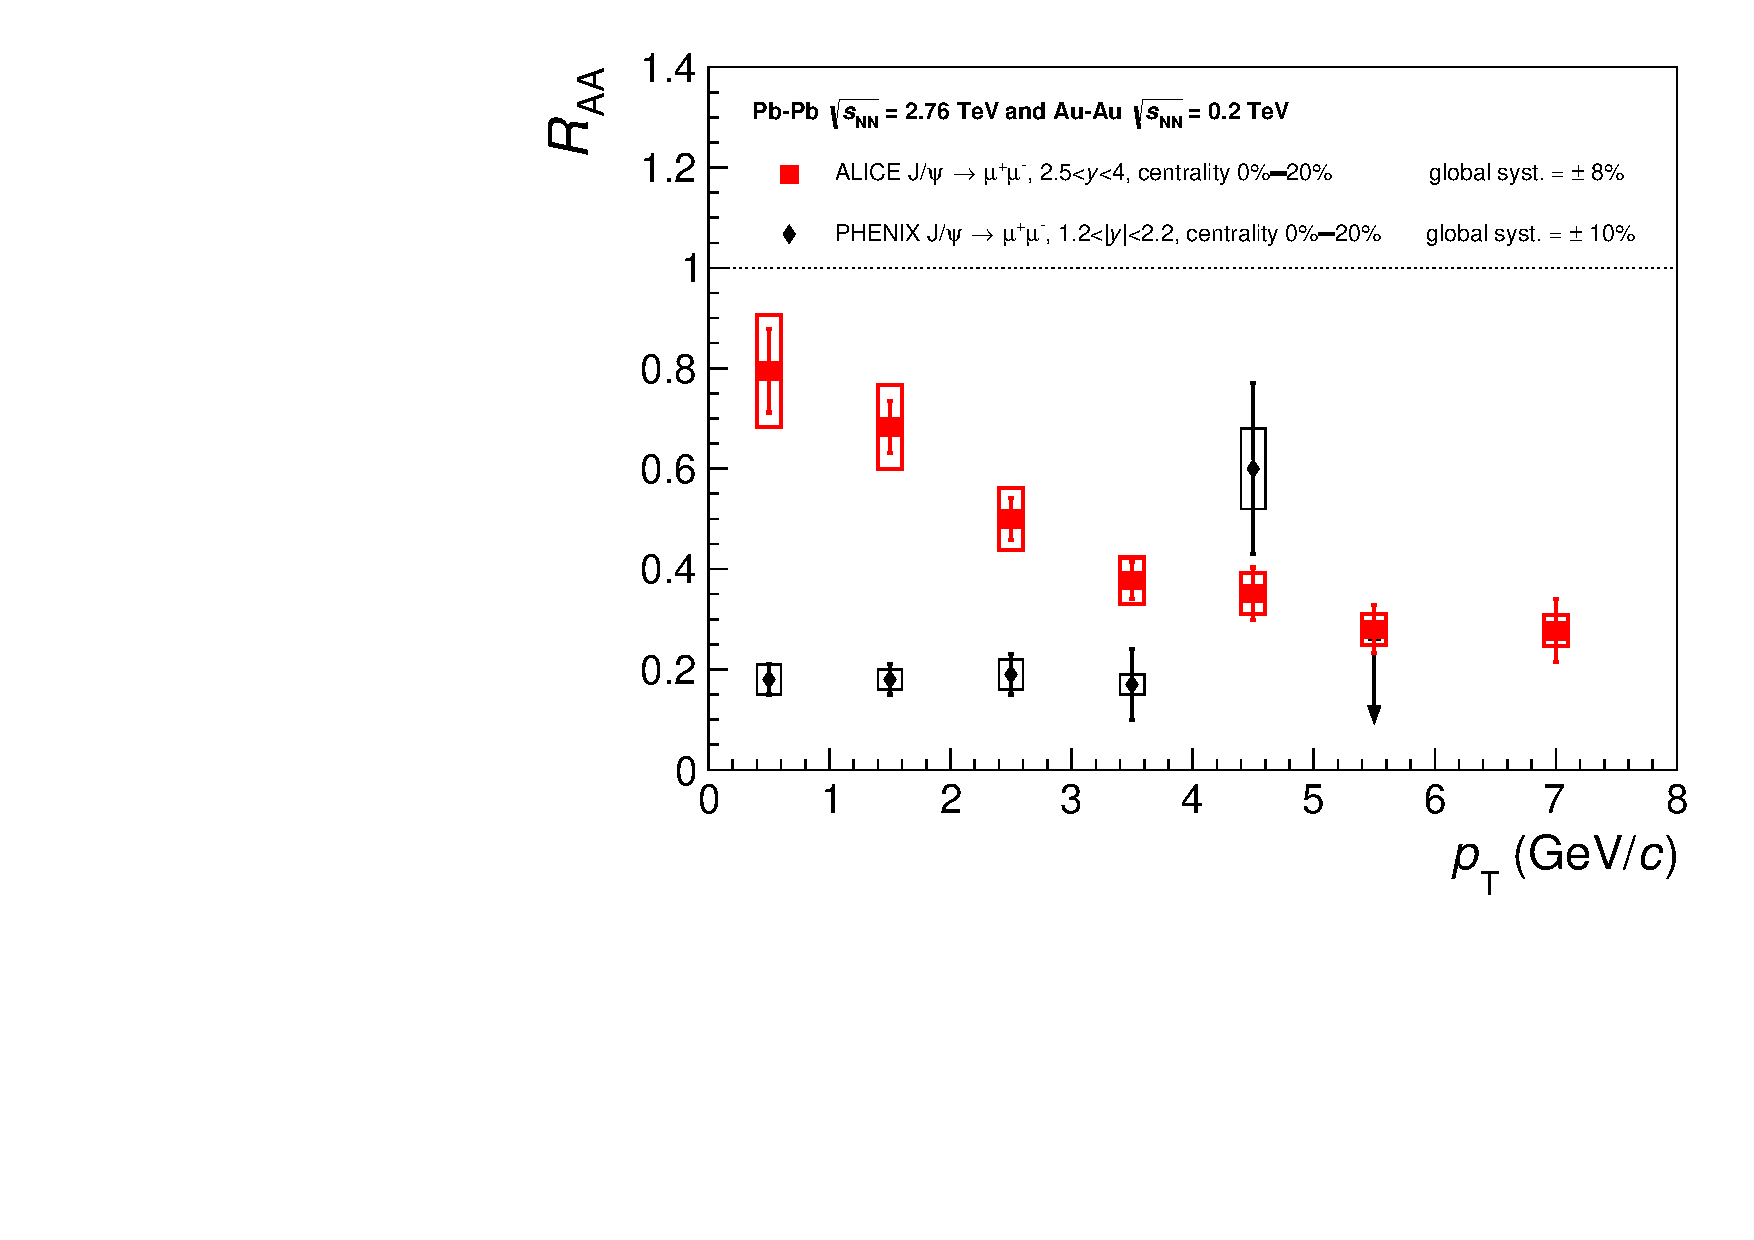
\includegraphics[width=0.49\linewidth,keepaspectratio]{quarkoniafigs/RAAPtvsModels2.pdf}
\caption{ \label{fig:KS:RaaPt}
(Left): Transverse momentum dependence of \Jpsi\ \Raa\ measured by ALICE~\cite{Abelev:2013ila} (0--90\,\% centrality) and by CMS~\cite{Chatrchyan:2012np} (0--100\% centrality) in \PbPb\
collisions at $\rootsNN = 2.76$\TeV.
(Right): Transverse momentum dependence of the \Jpsi\ \Raa\ measured by ALICE in the 0\%--20\% most
central \PbPb\ collisions at 2.76\TeV\ compared to PHENIX~\cite{Adare:2011yf}
results in the 0\%--20\% most central \AuAu\ collisions at 200\GeV. Reproduced from~\cite{Abelev:2013ila}}
\end{center}
\end{figure}

In Fig.~\ref{fig:KS:RaaPt} the inclusive \Jpsi\ $R_{\rm AA}$ dependence on transverse momentum is presented: (left) integrated over centrality, and (right) for the top 20\,\% of central collisions, compared to the PHENIX result. In both centrality ranges at the LHC the \Jpsi\ is little suppressed at low \pt\ ($\Raa \approx 0.8$ at \pt\ 0--1~GeV) and much more strongly suppressed at $\pt > 5$~GeV ($\Raa \approx 0.4$ for centrality integrated data, $\Raa \approx 0.25$ for 20\,\% of most central collisions). The comparison to the \pt\ dependence measured at RHIC, where the \Jpsi\ is strongly suppressed already at low \pt\ and no further decrease od \Raa\ is observed with increasing \pt, confirms the new regime of \Jpsi\ production achieved at the LHC. These results are qualitatively consistent
with the expectations of recombination approaches such as~\cite{Zhao:2007hh,Zhou:2013aea,Liu:2009nb}, while a quantitative interpretation of this result will require
a detailed understanding of cold-nuclear-matter effects. First results on \Jpsi\ production in \pPb\ collisions at the LHC have recently been published~\cite{Abelev:2013yxa,Aaij:2013zxa}, allowing the direct measurement of such effects.

\subsection{Charmonium Elliptic Flow}

For the study of the \Jpsi\ production mechanism, in addition to the $R_{\rm AA}$, the precise measurement of the elliptic flow is an important ingredient. Like for open charm production (Sec.~\ref{subsecks:heavyflow}) the value of the elliptic-flow parameter $v_2$ reflects the degree of thermalization of charm quarks. If charm quarks participate in the collective expansion of the medium, as suggested by the observed elliptic flow of open charm mesons, \jpsi\ produced by recombination should acquire the elliptic flow of these charm quarks.

At RHIC the \Jpsi\ elliptic flow was measured by the STAR collaboration~~\cite{Adamczyk:2012pw}. The $v_2$ for Au--Au collisions at highest RHIC energy $\rootsNN = 200$~GeV is compatible with zero, however, with rather large uncertainties, which do not allow a definite conclusion. At the LHC, ALICE has reported a non-zero \Jpsi\ $v_2$ with a significance of 2.1 standard deviations~\cite{ALICE:2013xna}. This result is presented in Fig.~\ref{fig:KS:v2ptcomp} as the transverse-momentum dependence of the \Jpsi\ $v_2$ for Pb--Pb collisions at $\rootsNN = 2.76$~TeV in the centrality range 20--60\,\%, i.e. semi-central collisions, where a maximal effect is expected. The measurements are compared with two model calculations~\cite{Liu:2009gx,Zhao:2012gc} which include the \Jpsi\ production via c$\overline{\rm c}$ recombination. Both are compatible with the experimental data within the current large uncertainties.

\begin{figure}[!ht]
\begin{center}
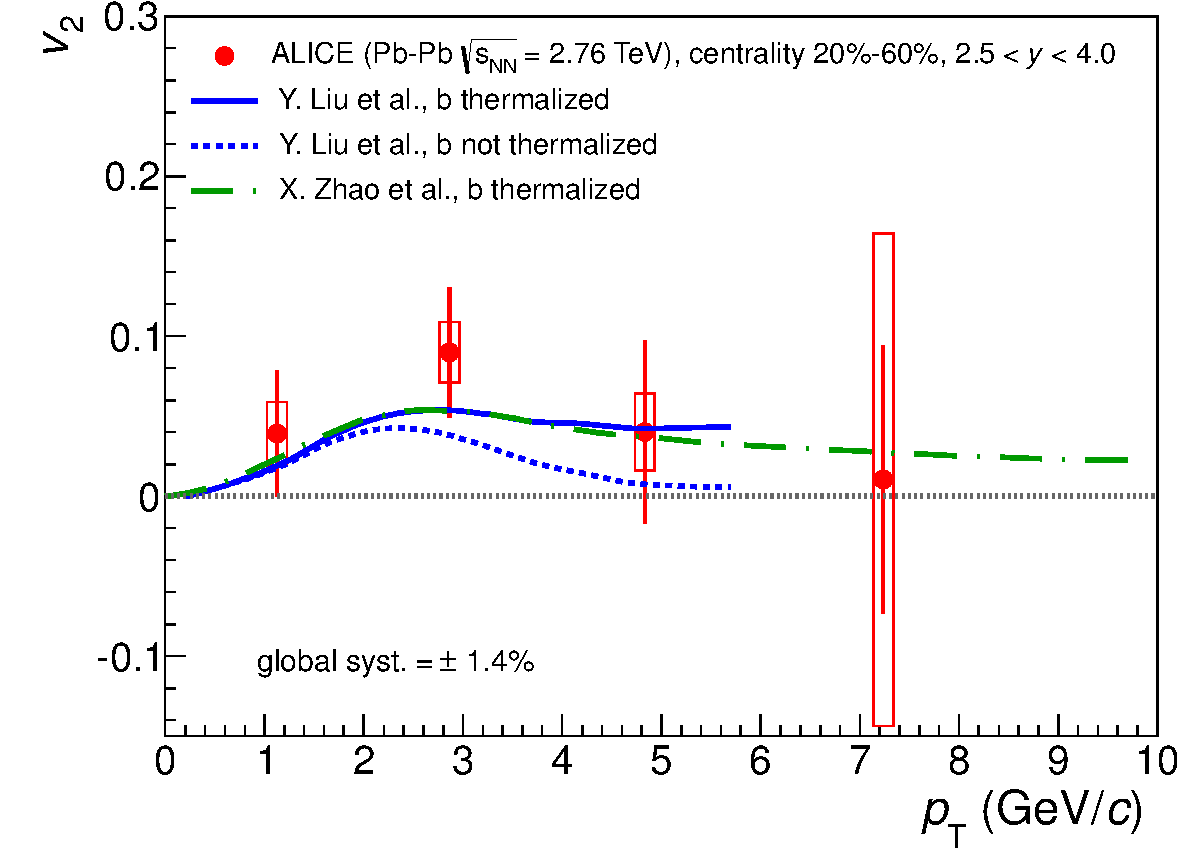
\includegraphics[width=0.49\linewidth]{quarkoniafigs/prl_fig4-eps-converted-to.pdf}
\label{fig:KS:v2ptcomp} 
\caption{Inclusive \jpsi\ \vtwo\
for \PbPb\ collisions with 20--60\% centrality at $\rootsNN = 2.76$\TeV\ as a function of \pT.
Also shown are the calculations from two transport models~\cite{Liu:2009gx,Zhao:2012gc}.
Reproduced from~\cite{ALICE:2013xna}}
\end{center}
\end{figure}

 Since, as discussed above, a fraction of \Jpsi\ originate from B-hadron decays, the results of model calculations depend on whether or not b quarks are assumed to be also thermalized. The model~\cite{Liu:2009gx} is presented for the two assumptions, showing a difference at higher \pt, where the B-decay fraction is larger and \Jpsi\ production by recombination is less important. The $v_2$ data prefer the version with thermalized b quarks, however, future precise measurements together with the access to higher \pt\ will shed more light on the question of b-quark thermalization. In addition, at high \pt\ initially produced \Jpsi\ in semi-central collisions may acquire a positive $v_2$ due to the different path length in the in-plane and in the out-of-plane directions, implying less dissociation in shorter in-plane path than in the out-of-plane direction. The various contributions can possibly be disentangled
by future precise studies of the \pT\ dependence of \Jpsi\ suppression and elliptic flow.

\subsection{Upsilon Suppression}

CMS measurements have provided the first high statistics data on \PgU\ production in heavy-ion collisions~\cite{CMS_Y_2010}. The three measured \PgU\ states have similar production and decay kinematics but different binding energies, and are therefore well suited to study in-medium heavy-quarkonium dissociation.
Uncertainties due to cold-nuclear-matter effects and to feed-down from higher mass states are less important for the \PgU\ family, compared to the situation of charmonium measurements. Since regeneration of \PgU\ states is presumed to be negligible, their suppression is expected to reflect pure dissociation processes. A complete understanding of the latter will also help the study of charmonia, where both mechanisms are present.

%Figure~\ref{fig:KS:mass} shows the invariant-mass spectra of $\mu^+\mu^-$ pairs produced in pp (left) and in Pb--Pb %(right) collisions obtained by CMS~\cite{Chatrchyan:2012lxa} at 2.76~TeV collision energy for both systems.
%For the \pp\ data, the excellent mass resolution of the CMS muon system
%allows a clear separation of the three \PgUn\ states. A similar mass resolution is achieved
%for \PbPb\ collisions.
Already the first invariant-mass spectra of $\mu^+\mu^-$ pairs produced in pp and in Pb--Pb collisions obtained by CMS~\cite{Chatrchyan:2012lxa} indicates
 a strong suppression of the \PgUb\ state is for \PbPb\ collisions, and the \PgUc\ state is even no longer visible above the combinatorial background. These results confirm the first \PgU\ measurement reported in~\cite{CMS_Y_2010}, and are in qualitative agreement with the expected \PgU\ suppression pattern as a function of the \PgUn\ binding energy.

%\begin{figure}[!ht]
%\begin{center}
%    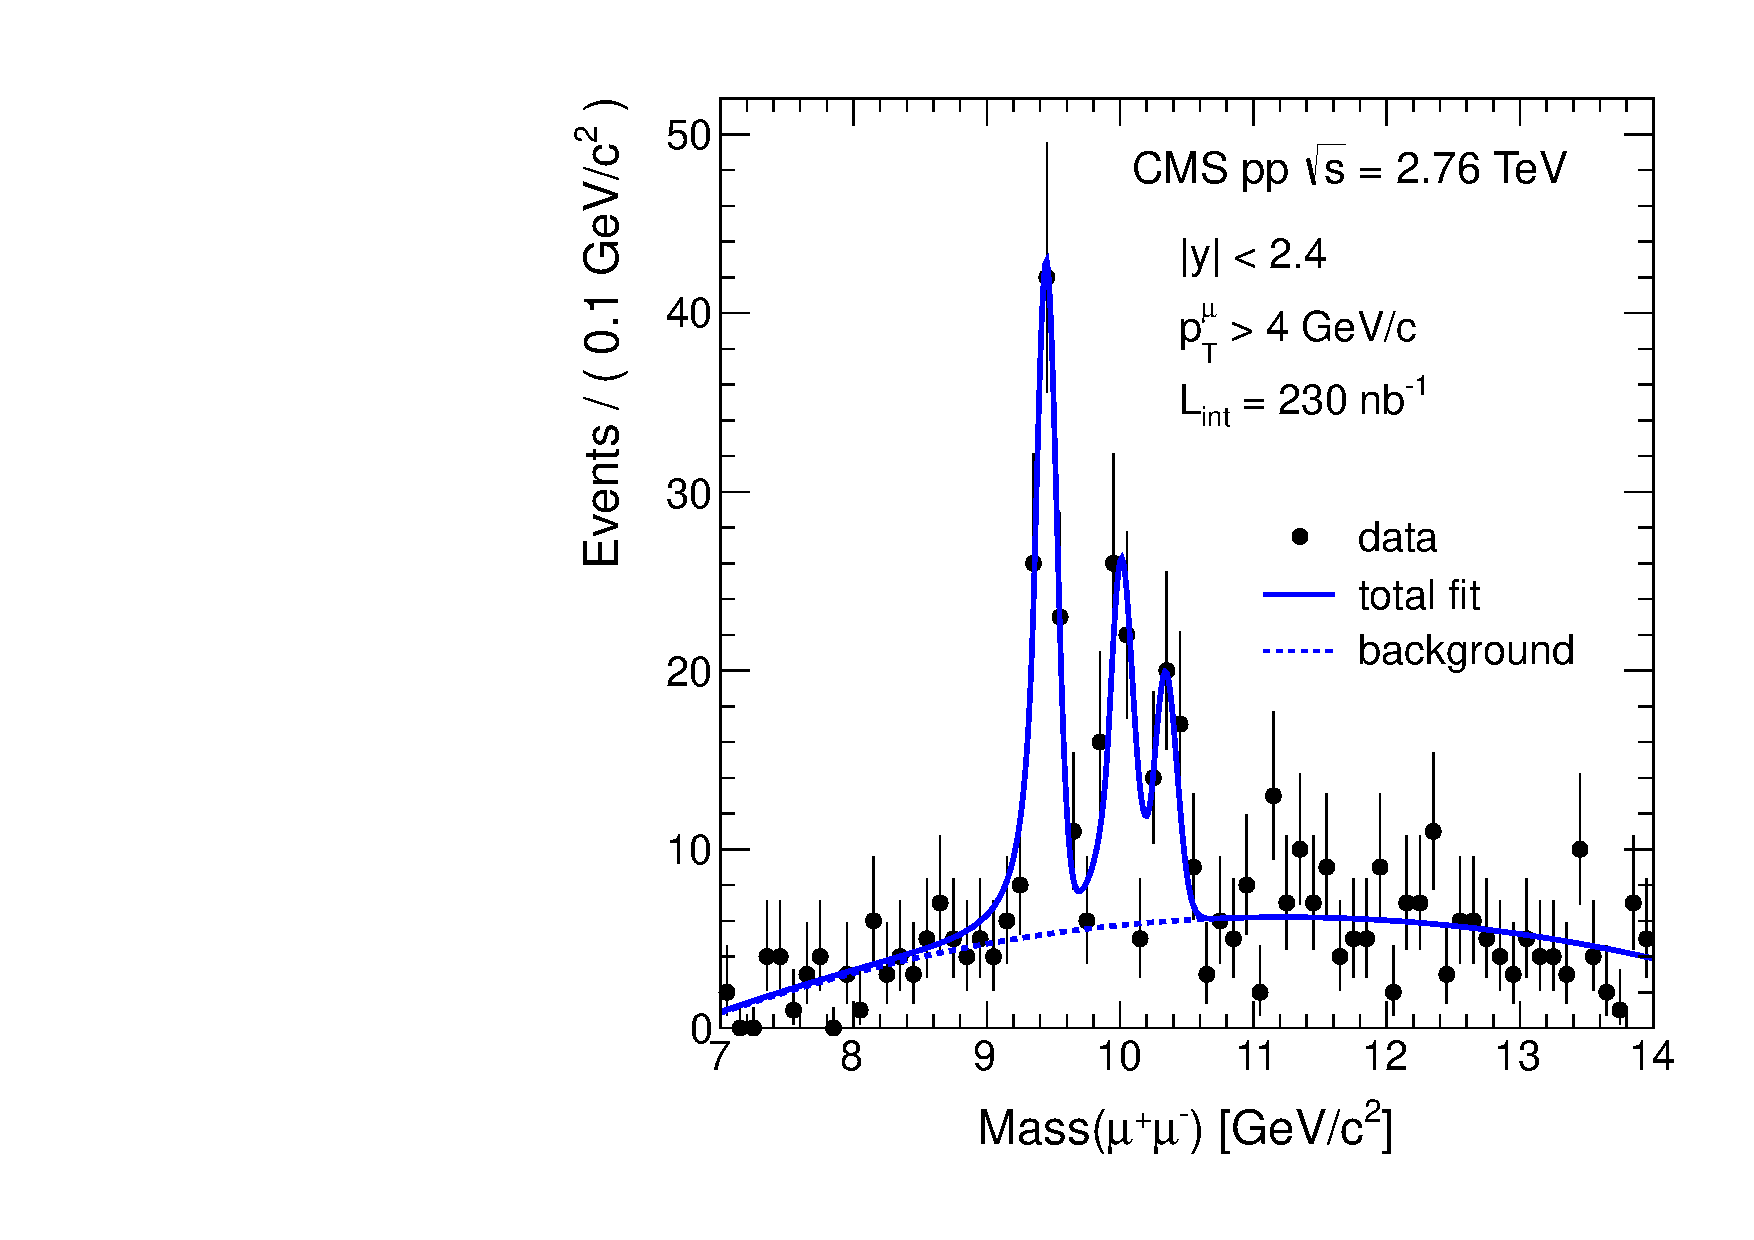
\includegraphics[width=0.45\textwidth]{quarkoniafigs/ppFitPt4Erf}
%    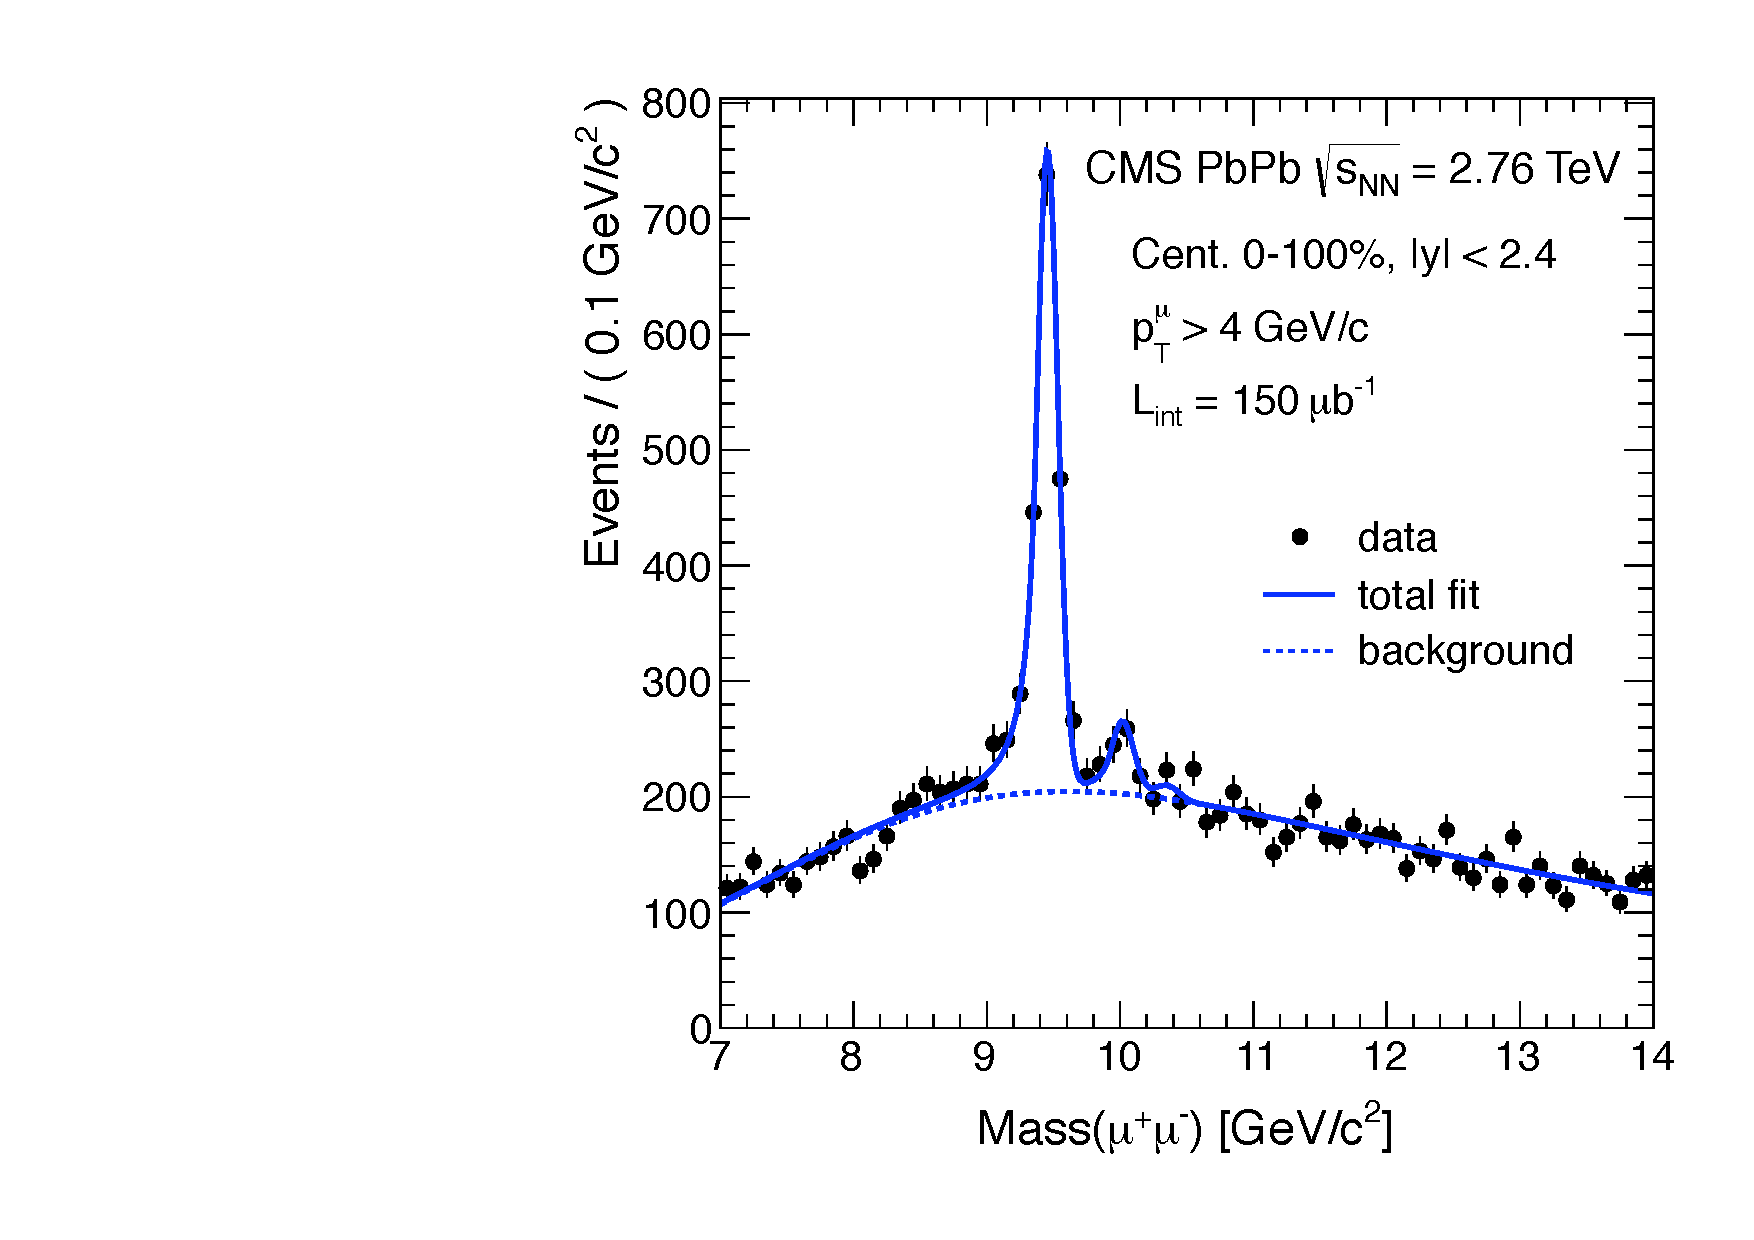
\includegraphics[width=0.45\textwidth]{quarkoniafigs/hiFitPt4Erf}
%    \label{fig:KS:mass}
%    \caption{Dimuon invariant-mass distributions in \PbPb\ (left) and \pp\ (right)
%at $\rootsNN = 2.76$\TeV. The lines show simultaneous fits to both
%data-sets for signal-and-background (solid) and background-only (dashed) contributions.
%Reproduced from~\cite{Chatrchyan:2012lxa}}
%\end{center}
%\end{figure}

From the \PbPb\ and \pp\ measurements the nuclear modification factor \Raa, characterizing the \PgU\ suppression,
can be calculated. The following centrality-integrated \Raa\ values were obtained for the different \PgUn states:
\begin{eqnarray}
\Raa (\PgUa) &=& 0.56 \pm 0.08\,\text{(stat.)} \pm 0.07\,\text{(syst.)} \,, \nonumber \\
\Raa (\PgUb) &=& 0.12 \pm 0.04\,\text{(stat.)} \pm 0.02\,\text{(syst.)} \,,  \\
\Raa (\PgUc) &=& 0.03 \pm 0.04\,\text{(stat.)} \pm 0.01\,\text{(syst.)} .  \nonumber
\end{eqnarray}
The statistical significance of the \PgUc\ signal is less than one standard deviation.
For the \PgUa\ state, there are significant feed-down contributions from the higher-mass bottomonia that may account for approximately 50\,\% of the yield~\cite{Affolder:1999wm, Aaij:2012se}.
This means that directly produced \PgUa\ state is probably largely unsuppressed, with
the observed \PgUa\ \Raa\ value essentially caused by the dissociation of the higher-mass excited states.


\begin{figure}[!ht]
\begin{center}
%   \includegraphics[width=0.45\textwidth]{qqbarfigures/chi2VsCent}
   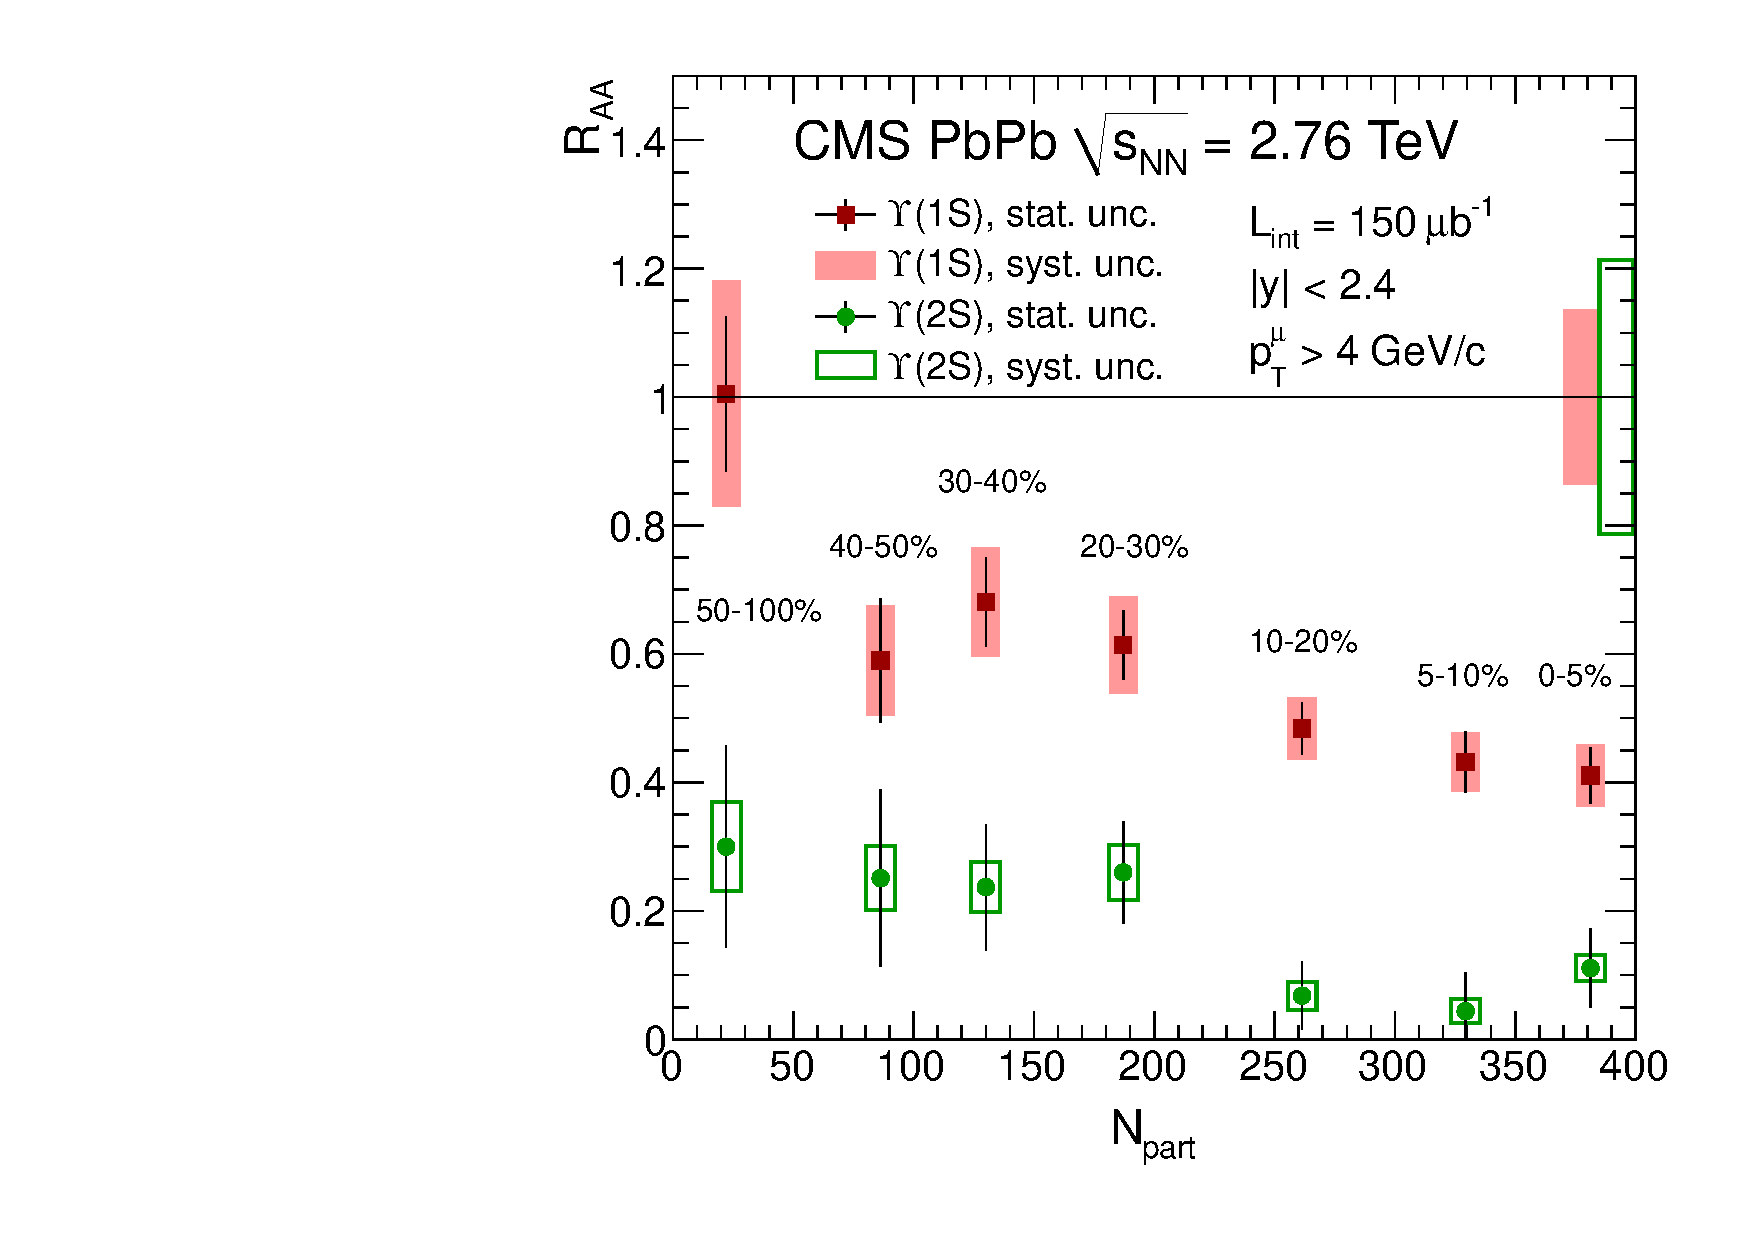
\includegraphics[width=0.49\textwidth]{quarkoniafigs/RaaPt4.pdf}
   \label{fig:KS:centrality}
  \caption{
%(Left): Centrality dependence of the \PgUa\ and \PgUb\ double ratios
%for 2.76\TeV\ \PbPb\ collisions.  (Right):
Nuclear modification factor \Raa\ for $\PgUa$ and $\PgUb$ as a function of $N_{\rm part}$ for $\rootsNN = 2.76$~TeV \PbPb\ collisions. Bars show statistical uncertainties, while the boxes around the points show systematic uncertainties. Common, centrality-independent uncertainties are represented by the boxes at unity. Reproduced from~\cite{Chatrchyan:2012lxa}}.
\end{center}
\end{figure}

The \PgUa\ and \PgUb\ suppression in terms of \Raa\ as a function of centrality expressed as $N_{\rm part}$
is shown in Fig.~\ref{fig:KS:centrality}.
%Here the relative suppression of \PgUa\ and \PgUb\ is characterized by
%the double ratio \linebreak $({\PgUb/\PgUa})_{\rm PbPb}/({\PgUb/\PgUa})_{\rm pp}$
%(Fig.~\ref{fig:GR:centrality}~(left) and the absolute suppression
%of the two states is shown as \Raa\ vs centrality (Fig.~\ref{fig:GR:centrality}~(right)).
The \Raa\ is strongly falling with increasing collision centrality
for both the \PgUa\ and the \PgUb, with a much stronger suppression for latter.
Overall, the data qualitatively exhibit the \PgUn\ suppression pattern
expected based on the hierarchy of binding energies. Although, the most peripheral bin
is rather wide (50--100\,\%), it is interesting to observe a strong suppression of the
\PgUb\ already for these centralities. 

ALICE and ATLAS are pursuing similar investigations of the \PgU\ family, and they have also presented their preliminary results.
Future high statistics \PbPb\ measurements
should elucidate the onset of the \PgU\ suppression in the most peripheral collisions,
in combination with information on \PgU\ production obtained from
studies of \pPb\ reference data, where the first results have been already reported.


